\chapter{Method, Design, and Implementation (3468/3500)}
\section{Overview, Theory \& Principles}
% Talk about how this works (decode audio, extract features, measure similarity, interpolate) as a general overview
The system I have designed provides interpolative playlist generation based on sets of data calculated about each song in the user's media library. The process begins by running the \executable{extractor} program on each of the files in the media library, which begins the process of extracting data about each song known as \emph{features}. These features, calculated from the audio data itself, aim to be an absolute measure of the sound (or \emph{timbre}) of the audio, by using statistical functions to gain values based on psychoacoustics. That is to say, ideally, the extracted features become an absolute measure of the timbre of the song, such that two songs with similar features will sound similar. Once these features have been extracted and stored, the \executable{generator} program reads the stored feature vectors into memory and generates a playlist by measuring the distance between the feature vectors, hence giving the \emph{similarity} between songs.

When measuring the similarity between songs, \executable{generator} biases the distance between songs according to a set of \emph{feature weights}, which are a measure of how important each of the features are towards an overall accurate similarity metric. The weights themselves are `trained' by analysing the output of a quiz (\executable{listenertest.rb}), asking the user of the system to pick the two most similar from three clips of songs from the library, a technique suggested by \citet*{Novello2006}. This both allows the system to train itself as to which features are important, but also later assess its own output (with the \executable{evaluate.rb} program) based on how well the similarity metric matches up with the answers given in the quiz.

Interpolative playlist generation involves the user inputting a set of \emph{key songs} and an amount of tracks to add. The system then, using the similarity measure, `fills the gaps' with tracks creating a smooth musical transition in genre between the keys. For example, if asked to interpolate one song between a blues and a hip-hop track it may pick a rhythm-and-blues track, in order to create as smooth a transition as possible. As well as selecting the `best' tracks to create the playlist, the generator also obeys rules of good playlist writing, such as not having songs by the same artist close to each other in the playlist (to add variety to the playlist). Appendix \ref{app:system_diagram} (page \pageref{app:system_diagram}) shows the conceptual layout of the system.
\begin{figure}[ht]
	\caption{Key to mathematical symbols}
	\begin{tabular}{l l}
		$\oplus$		& The exclusive OR operator \\
		$a$				& The vector containing amplitudes for each bin returned from the FFT \\
		$A$				& The vector of feature blocks for song $A$ \\
		$A'$			& The vector of sorted blocks in song $A$ \\
		$f$				& The feature vector for each block \\
		$f_n^{A_{i}}$	& The feature $n$ of song $A$, block $i$ \\
		$F$				& The vector containing frequencies of each bin of $a$ \\
		$g_{i,j}(A,B)$	& The distance between block $i$ of song $A$ and block $j$ of song $B$ \\
		$g_{s,s}$		& The distance between the song feature vectors of song $A$ and song $B$ \\
		$N_B$			& The number of bins returned by the FFT \\
		$N_F$			& The number of features in the vector \\
		$N_G$			& The number of blocks in song $A$ or $B$ (whichever is less) \\
		$N_R$			& The number of results from listener testing \\
		$N_S$			& The number of samples in one window \\
		$s$				& The vector containing signal data for one window \\
		$sgn()$			& Function returning 1 if positive, 0 if negative \\
		$w$				& The feature weights vector \\
		$W_S$			& The weight for the song block \\
		$W_B$			& The overall weight for the song blocks \\
		$v_i(A)$		& Sorting value for block $i$ of song $A$ \\
	\end{tabular}
\end{figure}
\section{Feature Extraction}
% the point of all these is that they each represent part of the sound of a song so that once you've got all the values out you have a measure of what it sounds like to your brain so a song that produces similar values by this measure are similar songs
When analysing an audio file to extract features, the system must first decode the compressed audio. This is performed by calling the external \software{gst-launch} program provided by \software{GStreamer} (\codepageref{SoundFile.cc}{21}) to decode to a temporary file, which is then read in using \software{libsndfile} (\coderef{SoundFile.cc}{45}); once the file has been fully processed, the temporary file is removed (\coderef{SoundFile.cc}{39}).

The audio file is read in 1024-sample (0.02 second) \emph{windows}, which are then passed to \software{FFTW3} (\codepageref{FFT.cc}{44}) to perform the Fourier transform. These two sets of data for each window are then passed to the relevant feature extractors, which return their features for each window (\codepageref{Features.cc}{94}). The features for each window, held by the \executable{FeatureSet} class, are then grouped into 150-window (3.5 second) blocks (\executable{FeatureGroup}s), where their mean, variance, skewness and kurtosis are calculated (\coderef{Features.cc}{29}). The reason for grouping the windows into these blocks is two-fold: first, it provides a two-tiered feature vector to the similarity measure, as all windows are processed into one song-level block at the end of processing (\codepageref{extractor.cc}{119}), which can provide a rough but much less computationally expensive similarity measure; second, it cuts down on the amount of data stored for each track (and hence helps meet the requirement of not storing too much data) while still providing information on the change in features over the track, and allows the standardised moments to be easily calculated.
\begin{figure}[h]
	\centering
	\caption{A processing block from the beginning of \emph{Quick and to the Pointless} by \emph{Queens of the Stone Age}: It begins with ``Yeah yeah yeah yeah!'', the fourth ``yeah'' being overlaid with the entry of the guitar, with three claps towards the end.}
	\subfigure[Waveform (the signal read from the audio file)]{\label{fig:method:block:waveform}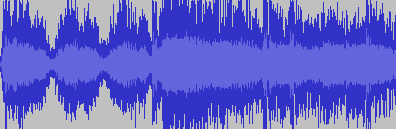
\includegraphics[width=0.5\textwidth]{method/waveform}}
	\subfigure[Spectrogram (a graphic representation of the spectrum returned by \software{FFTW3})]{\label{fig:method:block:spectrogram}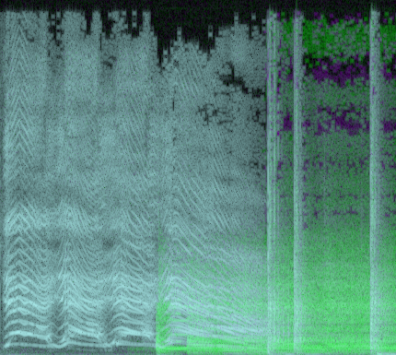
\includegraphics[width=0.5\textwidth]{method/spectrogram}}
	\label{fig:method:block}
\end{figure}
\subsection{Standardised Moments}
For each feature extracted the mean, variance, skewness and kurtosis over each three second block are calculated. It is these four values that are then used in the similarity measure, as it is unnecessary to store the output of each feature extractor for each window (and the amount of data would exceed what was set out in the specification, page \pageref{text:spec:requirement:data}). These values show how each feature for each window changes over the course of a block: variance describes how much the values change; skewness, how asymmetrical the data set is; and kurtosis, the `peakedness' or `flatness' of the data set \citep{Siegrist2007}.
\subsection{Signal Descriptors}
Signal descriptors are values which are calculated from the values of the audio data itself and tend to be values based on the periodicity or short-time amplitude of the signal. They are aggregate functions working directly on values stored in the audio files, and as of such are much less computationally expensive than the spectral descriptors, which require the output of an FFT. As is shown by figure \ref{fig:method:block:waveform}, it is easy to see the changes in amplitude, shape and periodicity as a whole from the waveform, but discerning polyphonic events is difficult (the fourth ``yeah!'' is almost completely obscured by the entry of the guitar).
\subsubsection{Zero Crossing Rate}
\begin{equation}
\mathit{Zero Crossing Rate} = \frac{1}{N} \sum_{i=0}^{N-2} sgn(s_i) \oplus sgn(s_{i+1})
\label{eq:zero_crossing_rate}
\end{equation}

The zero crossing rate is the number of times the signal passes from positive to negative or vice versa; it can be used as primitive pitch detection algorithm, and has been used successfully in the classification of percussive sounds \citep{Gouyon2000} and speech recognition[REF], due to the fact that it tends to be higher and unstable during the attack period of a sound \citep{Schwarz2004}.
\subsubsection{First Order Autocorrelation}
\begin{displaymath}
\mathit{FirstOrderAutocorrelation} = \frac{1}{N_S} \sum_{i=0}^{N_S-2} s_i \cdot s_{i+1}
\label{eq:first_order_autocorrelation}
\end{displaymath}

Autocorrelation is a measure of how well the signal matches a time-shifted version of itself, and hence shows the `noisiness' of the signal. \citep{Wikipedia2007}. As with zero crossing rate, this is useful to find attacks as well as being a measure of the harshness of the timbre of the sound.
\subsubsection{Energy}
\begin{displaymath}
\mathit{Energy} = \frac{1}{N_S} \sum_{i=0}^{N_S-1} (s_i)^2
\label{eq:energy}
\end{displaymath}

Energy gives a linear measure of the total amplitude in each window, giving an approximation of the perceived `loudness' of the sound. This will be useful for determining the level of change in energy per block, and hence be a measure of the distinctiveness of beats.
\subsection{Spectral Descriptors}
Spectral descriptors use Fourier series (the output of a discrete Fourier transform); rather than working in the dimensions of amplitude and time, they output values from the dimensions of frequency and amplitude. Figure \ref{fig:method:block}, \vpageref{fig:method:block}, shows the data analysed for one block of audio for both the spectral and signal descriptors. Spectral descriptors, working in the frequency domain, aim to represent features of the timbre of the sound, with the higher statistical moments looking at the change in timbre over blocks.
\subsubsection{Linear Regression}
\begin{equation}
\beta = \frac{n \sum (xy) - \sum x \sum y}{n \sum x^2 - \sum x^2}
\label{eq:linear_regression}
\end{equation}

Linear regression finds the line of best fit through a set of data. This statistical approximation has been used to find the gradient ($\beta$) of the spectrum, which is a measure of the ratio of high-frequency to low-frequency component of the sound and hence the timbre. With this feature the variance will most likely be a valuable similarity measure, as it will show the smoothness of timbre - long sustained notes will have low variation in linear regression, fast or noisy music will have a large variance.
\subsubsection{Centroid}
\begin{equation}
\mathit{SpectralCentroid} = \frac{\displaystyle \sum_{i=0}^{N-1} a_i f_i}{\displaystyle \sum_{i=0}^{N-1} a_i} 
\label{eq:spectral_centroid}
\end{equation}

The spectral centroid is analogous to the centre of gravity of a set of data if it were imagined to be a 2D shape \citep{Park2004}; it represents the average frequency weighted by amplitude, and hence where most of the energy of the signal lies. Psychoacoustically it is a measure of the perceived `brightness' of the sound, providing a better estimation of a `bright' sound than pitch \citep{Schubert2004}, and tending to rise for more intense sounds. This feature will represent the timbre of each block as a whole, and provide information on the change in timbre through the song.
\subsubsection{Smoothness}
\begin{equation}
\mathit{SpectralSmoothness} = \sum_{i=0}^{N-1} 20 \log a_i - \frac{20\log a_{i-1} + 20\log a_{i} + 20\log a_{i+1}}{3}
\label{eq:spectral_smoothness}
\end{equation}

Smoothness, also known as flatness, can be used to obtain a measure of the spectral envelope (the change in spectrum over time) of a sound \citep{Klapuri2003}. It is a measure of how spread out the signal is across the spectrum --- white noise, which has power at all frequencies, would have a smoothness of around 1; a sine wave, on the other hand, would have a smoothness of 0, as it is a single spike in the spectrum \citep{Peeters2004}. Using this, the smoothness will give a good measure of the noisiness and harmonicity of the signal.
\subsubsection{Spread}
\begin{equation}
\mathit{SpectralSpread} = \sqrt{\frac{\sum_{i=0}^{N-1} a_i (f_i - \mathit{SpectralCentroid})^2}{\sum_{i=0}^{N-1} a_i}}
\label{eq:spectral_spread}
\end{equation}

Spectral spread describes the variance of the signal about its spectral centroid \citep{Peeters2004}, and hence the perceptual `width' of the timbre. Orchestral or `full-sounding' tracks will have a large spread, whereas a monophonic or solo performance will produce smaller values.
\subsubsection{Dissymmetry}
\begin{displaymath}
\mathit{SpectralDissymmetry} = \sqrt{\frac{\sum_{i=1}^{N_B} a_i (F_i - \mathit{SpectralCentroid})^3}{\sum_{i=1}^{N_B} a_i}}
\label{eq:spectral_dissymmetry}
\end{displaymath}

Dissymmetry (or skewness) is a measure of how skewed the spectrum is about the spectral centroid, and hence the tilt towards high or low frequencies. Along with smoothness and spread, this is another extractor gaining values about the shape of the spectrum; in this case, a measure based on the harmonicity of the sound near the spectral centroid.
\subsection{Commentary}
For the system designed, eight feature extractors have been implemented, each aiming to be an absolute measure of a part of the timbre of a track, in order to later measure the similarity. The feature extractors used were chosen through evaluation of the development time alotted, processing time required and performance of the system. While it would have been possible to implement more, such as the MFCC used by \citet{Schnitzer2003} and \citet{Aucouturier2002a} or the range available with \software{Marsyas}, increasing the number of feature extractors would not necessarily increase accuracy, and would require more development and processing time.
\section{Similarity Measure}
\label{text:method:similarity_measure}
The similarity measure, performed by \executable{generator} (in \codepageref{Song.cc}{162} and \codepageref{Features.cc}{46}), works on the features stored by \executable{extractor}. When \executable{generator} is run, it begins by loading the analysis files / feature vectors for each of the songs in the media library (\codepageref{SongSet.cc}{21}). These are then normalised into the range 0--1, in order to avoid any feature having bias over others due to its values being larger (the difference between two centroids could be several thousand; when added to the distance between two linear regressions which are $-1$ to 1, the centroid would have much more effect on the similarity than the regression). When \executable{generator} is run with the \texttt{-s} command-line option, it performs a similarity measure against a specified track and every other track in the database, returning the top $n$ matches, so that the similarity measure can be tested alone from the playlist generation.

To compute the similarity between two songs, \executable{generator} computes the difference between two feature blocks using the following equation:
\begin{equation}
g_{i,j}(A,B) = \sum_{n=0}^{N_F-1} w_n | f_n^{A_i} - f_n^{B_j} |
\label{eq:feature_block_distance}
\end{equation}
\begin{center}
	\small \textit{(where $i$ and $j$ are $s$ for the song blocks of song $A$ and $B$)}
\end{center}

That is, the total of the absolute value of each feature subtracted from the corresponding feature in the second block, multiplied by the corresponding weight.

\note{how does changing block size affect similarity measure}
As the feature blocks extracted from the audio are sequential three-second clips, the similarity measure is very dependant on both the tempo of the music and the order of the blocks when compared to another song. If the beats happen to fall at the same rate as the blocks are extracted (roughly 69 or 138bpm, the energy measure will be inflated and not match the `true' timbre. Likewise, the structure of the song will affect the features extracted as the timbre of the verse will be substantially different from the chorus (for example), therefore putting more emphasis on the order of comparisons. This has been overcome in two ways: first, the overall song feature block is the average timbre of the entire track, and hence is not affected by the structure of the song; second, four different methods of comparing the feature blocks have been implemented and evaluated, each with their own advantages for the overall similarity metric.

\label{text:method:comparison_methods}
\subsubsection{Ordered Comparison}
\begin{equation}
s_o(A,B) = W_S g_{s,s}(A,B) + W_B \frac{\sum_{i=0}^{N_G-1} g_{i,i}(A,B)}{N_G}
\label{eq:song_distance_ordered}
\end{equation}

The first algorithm implemented was the simple ordered comparison: block 1 in song 1 is compared to block 1 in song 2, block 2 to 2 and so on. This similarity measure will be strongly affected by the structure of the two tracks: if the same song is compared to one with three seconds of silence at the beginning, it will return a similarity much lower than it should. However, by being so reliant on structure, it will rank similar-structured songs as more similar, therefore possibly working better for already-similar tracks such as a set of tracks from the same album.
\subsubsection{Ordered Area Comparison}
\begin{equation}
s_a(A,B) = W_S g_{s,s}(A,B) + W_B \frac{\sum_{i=1}^{N_G-1} g_{i,i-1}(A,B) + \sum_{j=0}^{N_G-1} g_{j,j}(A,B) + \sum_{k=0}^{N_G-2} g_{k,k+1}(A,B)}{3N_G-2}
\label{eq:song_distance_ordered_area}
\end{equation}

The area comparison hopes to improve on the ordered comparison (\ref{eq:song_distance_ordered}) by additionally comparing the previous and next block from song B with song A, thereby comparing each block from song A with a nine second area in song B. Comparing songs in this way means that the comparison still takes structure into account, but is less reliant on the structural changes happening at the same time in two tracks for a low similarity measure. Additionally, by comparing three groups at once, the problems with the timings of the song aligning with the block boundaries are alleviated.
\subsubsection{Exhaustive Comparison}
\begin{equation}
s_e(A,B) = W_S g_{s,s}(A,B) + W_B \frac{\sum_{i=0}^{N_G-1}\sum_{j=0}^{N_G-1} g_{i,j}(A,B)}{{N_G}^2}
\label{eq:song_distance_exhaustive}
\end{equation}

Exhaustive comparison aims to get a `complete' comparison of the two tracks, by comparing each block from song A to each in song B, and hence is not affected by the structure of the song in any way. This is also the only comparison which takes the whole of both songs into account, regardless of length. This means that it will provide much better results than the other comparisons in the case of songs $A$ and $B$ having greatly different length, but will be the slowest of all comparisons to compute.
\subsubsection{Sorted Block Comparison}
In the sorted block comparison, the feature blocks from both songs are both sorted according to the sum of their normalised features:
\begin{equation}
v_i(A) = \sum_{n=0}^{N_F-1} f_n^{A_i}
\label{eq:feature_block_sorting_value}
\end{equation}

The songs are then compared in the same way as the ordered comparison:
\begin{equation}
s_s(A,B) = W_S g_{s,s}(A',B') + W_B \frac{\sum_{i=0}^{N_G-1} g_{i,i}(A',B')}{N_G}
\label{eq:song_distance_sorted}
\end{equation}

This approach is similar to the exhaustive comparison in that it is unaffected by structure, but provides a rough (and hence much less expensive) comparison between already similar blocks in the two songs (as they have been sorted by their total), meaning it will be focusing on much smaller differences between features, and hence work best for finding very similar tracks even if the structure is disparate.
\subsection{Commentary}
As it is unknown which way to compare blocks will result in the best overall performance, four different algorithms have been implemented and will later be evaluated. Although some algorithms may work better than others in specialisation it is beyond the scope of this project to explore using combinations of these algorithms for increased accuracy, and it will become difficult to create a testing mechanism with the kind of accuracy required to evaluate fine-tuning of the similarity measure such as this, though it would be considered as a future extension.
\section{Playlist Generation}
\executable{generator}, when run in playlist generation mode, is supplied with a list of key songs and a number of tracks to add between. Once the feature vectors have been loaded and normalised (see page \ref{text:method:similarity_measure}), the playlist generator creates a new empty playlist of the correct length, with the key tracks in position (stored as an array of \executable{PlaylistEntry}s, \codepageref{Playlist.cc}{60}). The \executable{PlaylistEntry}s hold arrays of tracks, sorted in descending order of their similarity to the `ideal' track for that position in the playlist, created by interpolating between the song feature block of the two neighbouring key tracks (\coderef{Playlist.cc}{28}). At this stage, the playlist holds the closest matches to the ideal tracks, ie.\ the `best' playlist. To avoid repetition of artist (and hence improve the ???[REF]), the playlist generator then groups together tracks by the same artist between the same two key songs (\coderef{Playlist.cc}{112}), and scores them based on how similar they are to their ideal track for that position in the playlist (\coderef{Playlist.cc}{33}). The track which is best for that position in the playlist is kept, and the others are resorted with the artist in question removed. This process is repeated until no tracks remain with the same artist, when the playlist is outputted as a list of files relative to the media library folder (the M3U format).

The similarity measure used when sorting the tracks based on their similarity to the ideal track works solely on the song features, in order to cut down on the processing required to generate a playlist. If the playlist generator were to sort using the similarity to a set of interpolated feature blocks, each song in the media library would have to be compared multiple times to the `ideal' feature blocks, and it would be very computationally expensive. When calculating the score of each track (when removing artists), the feature blocks are taken into account to obtain a better similarity metric, and an weight added to the song features ($W_S$) and feature blocks ($W_B$) to bias the scores so they are not too dissimilar between the two similarity metrics.

Interpolative playlist generation in this manner reduces the reliance on a highly accurate similarity measure, as the metric is `guided' between tracks. Also, as repeated artists are excluded from the playlist, often the most similar track is skipped in favour of one with a different artist. It is only important for the similarity measure to return tracks with a roughly similar mood and timbre, so as not not `stick out' in a playlist --- the variety created by such a method is more important than a highly accurate measure of distance between songs.
\section{Weight Optimisation}
\label{text:method:weight_optimisation}
As it is not completely understood how we perceive sound and music, feature extractors only work as a basic model to return statistics based on the timbre of the sound; it is therefore best to use a number of these models and let empirical evidence from testing `teach' the system which of these best represent measures which can determine the similarity of audio. It is important for the system to have a vector of weights, which bias the comparison of songs towards certain features, in order to gain a more accurate similarity measure. The weight vectors represent a set of ratios of how important each feature is to the overall similarity measure; some features will be more useful to the similarity measure than others, and biasing towards these will improve the performance of the system.

The weights are trained through analysis of a user's answers to a \emph{music quiz} (\codefilepageref{listenertest.rb}), which asks the user to pick which two of three tracks played are the most similar. The results are then analysed, increasing the relevant weights according to features which were similiar in the two tracks given, using the algorithm shown in \ref{eq:weight_optimisation_old}.
\begin{equation}
w_i = \sum_{n=0}^{N_R-1} 1 - |f_i^{K_n^s} - f_i^{S_n^s}|
\label{eq:weight_optimisation_old}
\end{equation}
\begin{center}
	\small \emph{(where $f_i^{K_n^s}$ is feature $i$ of the song block of key song $n$, $f_i^{S_n^s}$ being the given similar track)}
\end{center}

Training in this manner allows the system to learn which features are important based on the user's estimate of similar tracks. Due to the length of time required to gather results (playing three extracts takes 30 seconds each, so it is a slow and labourious process, though training need only be done once) and hence the small amount of training data possible, the system considers tracks on the same album to be similar (especially true in the case of a compilation album) and uses these to further train itself, though giving less emphasis to these results as they were not specified by the user.

In addition to using tracks from the same album a source of similar track data, it would be possible as a future development to also query existing symbolic systems such as \software{Last.fm} or \software{Ruffle} for similar tracks and use these for training, providing the similar tracks returned by those systems are present in the user's media library.

The results from the music quiz can be used both in training and in testing, to determine how well the system learns and how accurate the similarity measure is. When provided with the results of the quiz, the system adjusts the weights aiming to return results more similar to the ones provided; the `perfect' system would, after training, give results identical to the training set while still having the ability to generalise to other music not used in the training. Using this, it is possible to automatically evaluate the efficacy of the system based on how close its results are to the user's responses, before and after testing.
\section{Critique of Design and Implementation}
The overall design of the system meets the specification well; the intensive audio processing happens once and is stored, playlist generation then being a much less intensive (and hence faster) process. Data is summarised during processing, reducing the data storage (~20KB per song) and subsequent processing time. To aid debugging, a data viewer has been provided, which produces warnings about invalid numbers. In the similarity measure where it is unknown which algorithm will work best, four algorithms have been implemented and will later be tested. A method for training and testing the system based on a user's `expert' input has been detailed, aiming to train the weights and hence denote more or less important features to the similarity metric.

Due to the object-oriented approach to the structure of the code, it is easy to extend and adapt. Once such improvement which could be made would be to pre-calculate distances between every track in the library, greatly reducing the computation required to generate playlists, possibly allowing the playlist generation to run on a portable device such as an MP3 player.
